\documentclass[fleqn,10pt]{wlscirep}
\title{FLOW17 - or: "Flow with the Go" (working title)}
% We'll decide on a succinct title once the main message is abs. clear

% insert here the call for the packages your document requires
\graphicspath{{./Figures/}}
% \usepackage[latin1]{inputenc}
\usepackage{amsmath}
\usepackage{amsfonts}
\usepackage{amssymb}
\usepackage{url}
\usepackage{xspace}
\usepackage{textcomp}
\usepackage{xcolor}
\usepackage{varwidth}
\usepackage{todonotes}
\usepackage{caption}

% please place your own definitions here and don't use \def but \newcommand{}{}
\newcommand{\hl}{\textcolor{red!60}}
\newcommand{\CCS}{\textsf{CogCarSim}\xspace}
\newcommand{\nicewidth}{0.8\textwidth}
\newcommand{\halfnicew}{0.4\textwidth}
\newcommand{\tapprx}{\raisebox{0.4ex}{\texttildelow}}


\author[1,2*]{Benjamin Ultan Cowley}
\author[1,5]{Jussi Palom\"{a}ki}
\author[1,3]{Tuisku Tammi}
\author[1,3+]{Roosa Frantsi}
\author[1,4+]{Ville-Pekka Inkil\"{a}}
\author[1+]{Noora Lehtonen}
\author[1]{Pasi P\"{o}l\"{o}nen}
\author[1]{Juha Veps\"{a}l\"{a}inen}
\author[1,3,5]{Otto Lappi}
\affil[1]{Cognitive Science, Department of Digital Humanities, University of Helsinki, Helsinki, Finland}
\affil[2]{Cognitive Brain Research Unit, Department of Psychology and Logopedics, University of Helsinki, Helsinki, Finland}
\affil[3]{TRUlab, University of Helsinki, Helsinki, Finland}
\affil[4]{Digitalization, Finnish Institute of Occupational Health, Helsinki, Finland}
\affil[5]{Helsinki Centre for Digital Humanities (HELDIG)}

\affil[*]{ben.cowley@helsinki.fi}

\affil[+]{these authors contributed equally to this work}

\keywords{Flow, Skill Acquisition, Power law of practice, Visuomotor performance, Steering, Eye blink rate, Negative Feedback, Dopamine}

\begin{abstract}
Example Abstract. Abstract must be under 200 words and not include subheadings or citations. Example Abstract. Abstract must be under 200 words and not include subheadings or citations. Example Abstract. Abstract must be under 200 words and not include subheadings or citations. Example Abstract. Abstract must be under 200 words and not include subheadings or citations. Example Abstract. Abstract must be under 200 words and not include subheadings or citations. Example Abstract. Abstract must be under 200 words and not include subheadings or citations. Example Abstract. Abstract must be under 200 words and not include subheadings or citations. Example Abstract. Abstract must be under 200 words and not include subheadings or citations.


Keywords: Flow, Skill Acquisition, Power law of practice, Visuomotor performance, Steering, Eye blink rate, Negative Feedback, Dopamine
\end{abstract}
\begin{document}

\flushbottom
\maketitle
\thispagestyle{empty}


\section*{Introduction}

In many fields of human endeavour - such as music, art and sports - the skilful performance of a demanding task can elicit a self-reported state of `optimal experience' called Flow \cite{Csikszentmihalyi1975}. The conditions for Flow are: {\sf C1} task demands match skill at a high level of performance; {\sf C2} clear and personally significant goals; and {\sf C3} unambiguous feedback on goal achievement. When these conditions are met, an individual may enter a mode of high performance characterized by several phenomenological features: {\sf F1} total focus in the present moment, and concentration on what one is doing; {\sf F2} merging of action and awareness (being `one' with the task); {\sf F3} loss of reflective self-consciousness or a sense of effortlessness and automaticity; {\sf F4} a sense of personal control and confidence in one's skill; {\sf F5} positive affect, or an experience of the activity as highly intrinsically rewarding; {\sf F6} a distortion of temporal experience (time may seem to go either slower or faster than normal) \cite{Nakamura2002,Engeser2012intro,Keller2012}. Flow is evaluated as an emotionally positive or enjoyable experience, and has an autotelic quality, i.e. people want to do Flow-producing activities for their own sake.

The antecedent conditions ({\sf C1-3}) and phenomenological features ({\sf F1-6}) of Flow have been investigated for several decades, mainly using qualitative analyses of self-report data from participants engaging in natural everyday or expert performance \cite{Csikszentmihalyi1971,Moneta2012}. Understanding in detail the conditions, their specific effects on mediating mechanisms, and the way these mechanisms give rise to the Flow experience would be significant for enhancing well-being or performance (e.g. through better design of recreational tasks such as games \cite{Chen2007}, or development of coaching practices or concentraton techniques in sport \cite{Jackson1996}). This calls for a more controlled and quantitative approach to studying Flow, using experimental psychology \cite{Harris2017,Keller2008} and psychophysiology \cite{Peifer2012,Peifer2014,Wolf2015,Harmat2015,Labonte-LeMoyne2016} approaches.

This paper reports an experimental study on the connections between performance, psychophysiology and the self-reported phenomenology of Flow in a novel and demanding visuomotor task.

\todo[author=OL, inline]{TODO (BEN) anticipate MAIN RESULT and its IMPLICATIONS here?\\
 - power law of practice is found in much previous work on (visuomotor) skill acquisition \cite{Newell1982}?\\
 - ...}

\paragraph{Protocol and Research Questions.}

Participants learned to play a custom-made high-speed steering game (Fig.~\ref{fig:cogcarsim}), which was specifically designed to elicit Flow by balancing task demand with the displayed skill of the participant, and providing clear immediate feedback. The aim in the game was to drive through a course with randomly placed obstacles at the highest possible speed. The game always started at a fixed velocity which increased at a constant rate. Collision with obstacles reduced speed by a fixed amount, and caused the screen to flash (see Methods for units).
% Speed, measured in units per time step, started at 1.6 units/step and increased at a constant rate;
This design, inspired by psychophysical staircase methods \cite{Cornsweet1962}, ensured constant match between skill and demand at the participant's level of performance. The outcome was measured by duration of the trial (shorter duration = faster average speed = better), displayed to the participant at the end of each run.

\begin{figure*}[!ht]
	\centering
	\includegraphics[width=\linewidth]{Screenshot_cogcarsim}
	\caption{The high-speed steering task. The participant steers the blue cube to avoid ostacles on the track. The game was designed to continually adapt the difficulty level (speed) to the participant's skill - one of the key antecedents of Flow.}
	\label{fig:cogcarsim}
\end{figure*}

Nine participants (6M, 3F) played the game in eight sessions over a period of 2-3 weeks, one session per day, 5 runs per session (each about 2-4 min duration, depending on performance), for a total of forty runs. Based on extensive informal piloting, we judged that about 2hr of driving time are sufficient to learn reasonable proficiency in this task, with no ceiling effect. The 10 item Flow Short Scale \cite{Engeser2008} was filled after each run to probe self-reported Flow in the task. Physiological data were recorded, during task and five minutes of baseline, in sessions one and five-to-eight.

This design allowed us to explore the following Research Questions:
\begin{enumerate}
	\item RQ1. How does performance change over time (what is the shape of the `learning curve')? Specifically, does performance in the game improve, and does improvement follow a power law of practice?

	\item RQ2. How is trial-wise Flow self-report related to performance? Specifically, is performance improvement across the whole experiment (i.e. learning) accompanied by higher levels of self-reported Flow (from hereon simply `Flow')?

	\item RQ3. Are there identifiable physiological markers of Flow and/or physiological measures that are predictive of task performance? Specifically, spontaneous eye blink rate (sEBR) was of interest in our reinforcement-based learning task, as it has a putative association with striatal dopamine \cite{Slagter2012}. Thus, we focus on this measure in the Results -- although we measured a number of physiological signals, the others will be analyzed and reported separately.

\end{enumerate}

\section*{Results}
% We should aim to make results understandable without the detailed methods which will be placed at the end
All participants completed the task (40 runs in total). Average run duration was 186s (SD 18.2s, min 162.2s, max 300.1s). Average number of collisions was 17.8 (SD 4.9, min 5, max 40). Average velocity of runs ranged between 1.37 and 2.54 units per step (mean 2.23, sd 0.19). Maximum instantaneous speed was 3.6 and minimum 1.06. The supplementary information provides comprehensive data on performance-related features, such as run duration; along with correlations between them.

\subsection*{RQ1}
{\sf RQ1} asks how does performance change over time: What is the form of the learning curve, does it consistently improve as a power law of (observed) practice \cite{Newell1982}? A power-law curve transformed to log-space will be linear. Thus, to investigate whether participant behaviour follows a power law, we fitted a linear model in log-log space (log-transformed dependent and independent variable) of run durations as a function of cumulative number of runs, for each participant separately. Fig.~\ref{fig:flowVperf} (panel A) shows this log-log performance data for each participant in each run. Blue dashed lines indicate the `ideal' learning according to the power law. Dispersion of points around the line indicates the divergence of each participant from ideal learning: points above the line indicate longer duration/worse performance than predicted by the learning curve, and vice versa.

% \begin{figure*}[!ht]
% 	\centering
% 	\includegraphics[width=\linewidth]{flowDeviation_all}
% 	\caption{The deviation score (observed run duration - predicted run duration) and Flow scores across all participants and trials.}
% 	\label{fig:grand_correlation_cogcar}
% \end{figure*}

\begin{figure*}[!p]
	\centering
	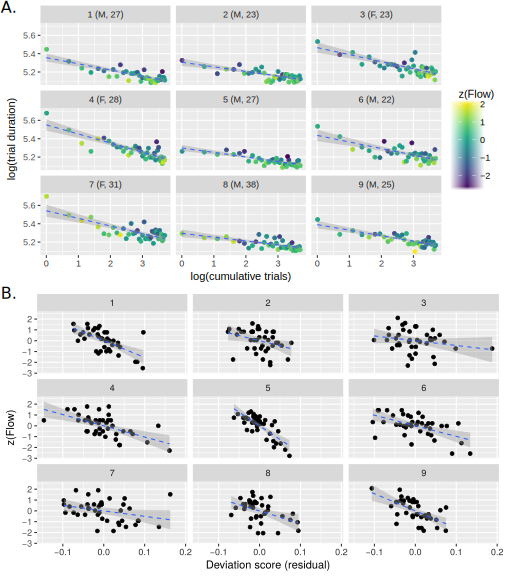
\includegraphics[width=\linewidth]{cogcar_main}
  % \includegraphics[width=\linewidth]{flowDeviation_panelsRL3}
	\caption{{\it Panel A}: Participant-wise data showing logarithm-transformed performance and Flow self-reports in the speeded steering task. Ordinate shows log-duration of runs, abscissa shows log-cumulative trial count. Dashed blue lines fitted to the data are `ideal' power-law learning curves, which transform to linear in log-log space.\\
  {\it Panel B}: Participant-wise deviation scores (observed run duration - predicted run duration) plotted against Flow scores for each participant, and fitted by linear models.}
	\label{fig:flowVperf}
	% \label{fig:indiv_correlation_cogcar}
\end{figure*}

All participant-specific models had negative slopes, which indicates that everyone improved (obtained faster run times) over time as they gained more game experience. The variation in intercepts suggests disparity in participants’ initial skill levels of the game task. The individual intercepts and slopes of the fitted log-log models are presented in Table~\ref{tab:LCxFlow}. A grand model (covering all the participants) was also fitted, and cumulative number of runs (i.e. the learning effect) explained 39.6\% of variance in run durations.

To confirm that the power law fit is a good approximation, we tested the fit of the power law model against a model of an exponential curve fit (see Supplementary Information for details). Both models had good fit, but the power law model was significantly better.
\todo[inline,author=BC]{JUSSI: check this and expand if needed.}

RQ1 can thus be answered: {\it the task was learned and the learning curve fit well to a power law model}. Given these positive answers, we may assume that the model provides a useful statistical estimate of performance expectation, i.e. how well the participants expect to perform can be estimated from the model.

\begin{table}[ht]
\centering
\caption{\label{tab:LCxFlow}Individual learning rate parameters (cols 1--3), Flow (cols 4--5) and perceived importance (P.I., cols 6--7) scores.}
\begin{tabular}{llllllll}
\hline
Participant & Intercept sec & Intercept log & Slope  & Flow mean & Flow SD & P.I. mean & P.I. SD \\
\hline
1                & 213     & 5.36      & -0.067 & 5.10      & .51     & 3.53      & .57     \\
2                & 202     & 5.31      & -0.049 & 5.18      & .39     & 4.29      & .47     \\
3                & 237     & 5.47      & -0.077 & 5.36      & .64     & 2.03      & .50     \\
4                & 257     & 5.55      & -0.099 & 4.40      & .39     & 4.12      & .46     \\
5                & 200     & 5.30      & -0.049 & 5.44      & .88     & 5.16      & .64     \\
6                & 230     & 5.44      & -0.071 & 5.22      & .82     & 4.33      & .56     \\
7                & 255     & 5.54      & -0.083 & 4.69      & .53     & 2.22      & .53     \\
8                & 198     & 5.29      & -0.041 & 4.94      & .90     & 3.67      & .70     \\
9                & 219     & 5.39      & -0.059 & 5.25      & .79     & 4.62      & .55     \\
\hline
Participant mean & 223     & 5.41      & -0.066 & 5.06      & 0.65    & 3.77      & .55    	\\
\hline
\end{tabular}
\end{table}


\subsection*{RQ2}
{\sf RQ2} asks: How is Flow related to performance? The points in each Fig.~\ref{fig:flowVperf} (panel A) subplot are coloured according to Flow self-reports made after each run, in a standardised range (i.e. original scores transformed to {\it z}-scores). The best Flow scores are green, the worst are red.

Since we have established that performance improves over sessions, we use session number as a simple proxy of performance improvement. Plotting the group-wise dispersion of Flow scores against sessions gives the result in Fig.~\ref{fig:FlowVssn}: clearly, there is no effect of session on group-wise Flow (Pearson's {\it r} = -0.12, {\it p} = 0.77 for median Flow and session).

\begin{figure*}[!ht]
	\centering
	\includegraphics[width=\nicewidth]{session_fss2}
	\caption{Violin plot representing participants' self-reported Flow in sessions 1-8 (Averages over five runs per session. The self-report items are given in Supplementary information, the scale was 1-7).}
	\label{fig:FlowVssn}
\end{figure*}

Next, we calculated Pearson correlation coefficient between median duration and median Flow, for each session. The relationship between duration and Flow was intermittently significant, but not with any particular trend. In the first session, the correlation was not significant ({\it r} = -.051, {\it p} = .90, N = 9). In contrast, the Pearson correlation coefficients were significant in training session 3 ({\it r} = -.71, {\it p} = .03), session 4 ({\it r} = -.74, {\it p} = .02), and session 6 ({\it r} = -.71, {\it p} = .03). These results suggest that higher Flow was sometimes associated with lower run durations (i.e. better performance), but not systematically. If we group sessions by condition (introduction=1, practice=2--4, main test=5--8), we can visualize the evolution of performance against Flow more clearly than by plotting each session individually, see Fig.~\ref{fig:FlowVdurXssn}.

\begin{figure*}[!ht]
  \centering
  \includegraphics[width=\nicewidth]{session_flowDuration_v3}
  \caption{Duration and Flow over sessions grouped: 1, 2-4 (training), 5-8 (physiological measurements), N = 72.}
  \label{fig:FlowVdurXssn}
\end{figure*}

Interestingly, in Fig.~\ref{fig:flowVperf} (panel A), we can see at a glance that the points lie above and below the log-transformed power-law line in good agreement with the level of experienced Flow: worse performing runs (data-point above the line) tend to be more red (Flow scores below the participant-wise mean), and better performing runs tend to be more green (scores above the mean). In other words, it seems that whenever participants were performing {\it better than predicted by the power-law line}, they were experiencing more Flow; and {\it vice versa} when they were performing worse than predicted.

We evaluated whether this effect was robust and statistically significant. For each participant and for each run (40 runs in total), we first subtracted predicted run duration (y-value of power-law performance line) from observed run duration, thus obtaining power-law model residuals. We refer to these within-participant run duration residuals as {\it deviation scores}, because they represent how much each observed run duration deviates from the duration predicted by the model. Then, we correlated the deviation scores with the participants' Flow scores. The stronger this correlation is, the more strongly high Flow scores are associated with run durations below the predicted performance line (i.e. {\it better than predicted results}), and {\it vice versa}.

Specifically, we first fit a linear mixed model with non-standardized Flow scores as the dependent variable, deviation scores as the predictor, and participant (numerical participant identifier ranging from 1 to 9) as a random factor with both random intercept and slope. This model was statistically highly significant ($\beta$ = -8, {\it t} = -4.36, {\it p} $<$ .001; see Fig.~\ref{fig:flowVperf} (panel B) with standardized Flow scores). The conditional pseudo-$R^2$ value for this model was .47, corresponding to a correlation of ~.68, and suggesting that about 47 per cent of the variability in Flow scores was explained. Thus, when the difference between observed and predicted run duration is negative (i.e. better than predicted performance), Flow scores are more likely to be positive with strong effect size.

Note that that there is no consensus on the best way to obtain {\it p}-values or estimates of effect sizes from linear mixed models. We have treated the {\it t} statistic as a {\it z} statistic using a standard normal distribution as a reference, and followed the method by Nakagawa {\it et al}~\cite{nakagawa2013general} to obtain pseudo-$R^2$ values. Another way to statistically evaluate the significance of these results is via the binomial distribution: The (two-tailed) probability of 9 negative slopes (should the probability of a negative slope per participant be 0.5, that is, fully random) is {\it p} = .007.

As can be seen in Fig.~\ref{fig:flowVperf} (panel B), the trend was clearly negative for 7 out of 9 participants, while for two participants, 3 and 7, the trend was similar but the relationship was weaker. Notably, these two participants also reported lower scores on perceived importance: mean scores for these participants were 2.03 and 2.22, whereas the overall mean was 3.77 (see Table ~\ref{tab:LCxFlow}). However, the overall interaction between participants’ scores on perceived importance and their deviation score was not statistically significant.

To sum, we observed that Flow was not only related to better performance (although not across all sessions), but {\it better (or worse) than predicted} (i.e. mathematically predicted) performance. Moreover, this effect seemed to be moderated by self-reported perceived importance of the driving task.


\subsection*{RQ3}
{\sf RQ3} asks if spontaneous eye blink rate is related to performance or Flow.

sEBR has a negative relationship to participant-wise learning curve (LC) slopes, as shown in Fig.~\ref{fig:EBRvLC}. The Pearson correlation for the relationship is of moderate strength, though non-significant ({\it r} = -.65 , {\it p} = .06). The LC slope of every participant was negative, which means we can say that the smaller the sEBR, the shallower the LC slope. Or, because slope and intercept are highly correlated, it is almost equivalent to say that smaller sEBR correlates with better initial performance.

Mean Flow scores are not related to sEBR, which can be easily seen from Fig.~\ref{fig:EBRvLC}. However, examining the Flow scores in Fig.~\ref{fig:EBRvLC} turns up an interesting relationship: the residuals of the fitted linear model (i.e. vertical distance of each data-point from the line) are {\it strongly} related to mean Flow scores (Pearson correlation {\it r} = -.85 , {\it p} $<$ .005). In other words, participants' mean Flow scores are strongly correlated with their observed deviation from the modelled linear relationship between sEBR and task learning (LC slope).
% data:  df$Flow and df$residual
% t = -4.3257, df = 7, p-value = 0.003456
% alternative hypothesis: true correlation is not equal to 0
% 95 percent confidence interval:
% -0.9685003 -0.4359516
% sample estimates:
% cor
% -0.8530842


\begin{figure*}[!ht]
	\centering
	\includegraphics[width=\nicewidth]{lcurve_sbr_flowRL2}
	\caption{Participants' median spontaneous eye blink rate plotted against the slope of their learning curve, and colored by their mean Flow scores. Linear model is depicted by the dashed line. Each point is labelled with the participant number (1..9) and exact mean Flow score (in parentheses).}
	\label{fig:EBRvLC}
\end{figure*}


%%%%%%%%%%%%%%%%%%%%%%%%%%%%%%%%%%%%%%%%%%%%%%%%%%%%%%%%%%%%%%%%%%%%%%%%%%%%%%%%
%%%%%%%%%%%%%%%%%%%%%%%%%%%%%%%%%%%%%%%%%%%%%%%%%%%%%%%%%%%%%%%%%%%%%%%%%%%%%%%%
%%%%%%%%%%%%%%%%%%%%%%%%     DISCUSSION    %%%%%%%%%%%%%%%%%%%%%%%%%%%%%%%%%%%%%
\section*{Discussion}
\todo[author=BC,inline]{TODO BC - write up properly:}

\textit{exploration of Flow and on-task learning (learning curve as opposed to pre- post)}
We present a longitudinal study of Flow in a game-like steering task, analysing learning curves of task performance, and sEBR.

\textit{game was fairly successful in eliciting Flow-like experiences (high baseline, score five out of seven)}
To induce Flow, the game was designed to hold the balance between skill and challenge constant: the difficulty of the game increased proportionate to the skill required to perform well. The results show the game was clearly Flow-inducing: grand average Flow was reported as 5.1 (out of 7) across sessions.

\textit{we do not see Flow increasing as you learn the game; it is not that when you play better you get more Flow}
We further found that Flow was not associated with gaining experience and skill in the game -- our participants did not report more Flow even as they learnt, session by session, to complete the runs faster. This is in line with the assumption that Flow is elicited by the balance of skill and challenge, instead of level of skill and challenge as such.

\textit{we are relating Flow to the learning mechanisms: the Flow reports across time are related via the learning curve (skill level)}
\textit{we do see that when you play better than expected, you report more Flow (but caution: direction on causation between Flow and performance unclear - does Flow lead to better performance or does better performance lead to higher (post hoc) self-reported Flow?)}
Moreover, higher Flow within a run (“local” Flow) was associated with shorter run durations compared with their learning curve predictions. In other words, while global average Flow remained relatively stable across all sessions, local Flow predicted better than expected performance within a run. This may reflect performance-enhancing effects of higher Flow, or alternatively that people are more likely to report higher Flow after finishing a more successful (rewarding) run.

To sum, learning to play the game did not itself increase Flow; rather, the game itself induced a fair amount of baseline Flow, and local variability around this baseline predicted better or worse than expected performance. Overall, then, global average Flow could be construed as the relatively stable Flow baseline induced by the game, reflecting skill-challenge balance, and local Flow as natural variability around this baseline.
\textit{this is a new or little used view in Flow research, looking at changes in or determination of Flow over different points in time as opposed to instantaneous or a static property}
A novel observation is that this variability is related to performance fluctuations around the expected performance (learning curve).
\textit{it's a good idea to look at Flow in relation to skill, across points in time...because we want to understand the mechanisms generating the experience (and the report of the experience)}

%%%% complete speculations - need some data to bolster these interpretations
% Beyond the described results, Figure~\ref{fig:flowVperf} (panel A) shows some more subtle patterns. Distribution of low-to-high Flow scores tend to change with the cumulative trials for participant 3, and inversely for participant 7. This could indicate increasing and decreasing motivation, respectively.
\todo[author=BC,inline]{Does model prediction capture participant {\it expectation} of performance? In the Discussion, we can speculate whether psychologically the changes in (self-reported) Flow are elicited by positive or negative violations of performance expectations.}


\subsection*{Learning, Flow, and models}
% Relation to previous Work on skill acquisition and Flow
\todo[author=OL,inline]{TO THINK ABOUT / DO SCHOLARLY WORK ON: how do we interpret Flow octant model "axes"? absolute or relative? relative to population or individual? how is the "origin" determined? (how did big C mean it and how did Keller and Landhauser interpet it? what about their "model"?)}

\textit{Here, we aim to provide empirical data to critically examine Flow models in the context of the larger question of Flow and learning, with particular focus on the Flow intensity model \cite{Keller2012} (as the octant/quadrant models have been well-criticised \cite{Moneta2012}).}

New psychological models of Flow \cite{Keller2012} (updating the classic channel and quadrant/octant models) show the conceptual advance of Flow research

One area of current interest is the relationship between Flow and task-relevant skill acquisition, which brings {\it on-task} learning into interaction with Flow. Psychological theory of Flow has dealt with state and trait models \cite{Moneta2012}, but to deal with on-task learning, Flow must be considered as a dynamic process (or linked to a dynamic process). Prior work has proposed such an account using (neuro)cognitive models of information-processing: including Marr's biobehavioural model \cite{Marr2001}; this lead author's model, which integrated elements from information theory to neurobiology \cite{Cowley2008}; or more recently, a descriptive model proposed by {\v{S}}imle{\v{s}}a and colleagues \cite{Simlesa2018} using a combustion-engine metaphor. However, these models have not yet been empirically tested.

One issue for linking Flow to learning is that existing Flow theory is not intrinsically built to handle the difference between simple and non-simple tasks: e.g. washing dishes versus driving cars
\todo[inline,author=OL]{Not clear which, if either, of these is complex (or simple)}
. If we allow that Flow can occur in all sorts of tasks
\todo[inline,author=OL]{not trivial,I think the Cszikzzz treatments are almost exclusively about 'complex' tasks?}
, and the tasks will be characterised by the depth of learning available, then it follows that Flow-as-a-process depends on the task `depth'.
To handle such distinctions, we must separate the phenomenal construct of Flow from the cognitive activity that gives rise to it. Some tasks require what we term `high-performance cognition' (HPC)
\todo[inline,author=OL]{If you want to introduce the HPC concept you need to define it; I don't think "feats of enactive cognition with high skill" is definite enough, and needs "enactive" to be defined}
, i.e. feats of enactive cognition with high skill, which are not synonymous with Flow despite sharing certain conditions. For this discussion, it is sufficient to consider that in HPC-class tasks, skill acquisition is required and is non-trivial for any duration of learning, i.e. HPC tasks must have a shallow learning curve (learning is slow). Importantly, the skill level does not quickly peak, such as with simpler tasks like washing the dishes, where Flow might be obtained but does not strongly interact with learning.
\todo[author=BC,inline]{Some semantic clashing between shallow learning curves (slow learning) and deep tasks (non-trivial skills), which are almost the same thing.}

\textbf{Nevertheless, the question of whether Flow is a state or a dynamic process, requires empirical testing}??

\todo[inline,author=OL]{I don't think Flow as a "state" or as a "process" is a really fundamental distinction; at any rate, it needs to be properly defined what is meant by it and what it implies}Flow-as-a-state leads us to expect that as skills improve and challenges are consequently raised, Flow self-report should increase over time. Consider a series of Flow-inducing sessions with skill acquisition, e.g. in a driving simulator. In such a `HPC' task, learning implies skill increase, which implies challenge increase, which together imply Flow increase. This is true whether we follow the classic Flow quadrant/octant model \cite{Massimini1988}, or Keller and Landhausser's \cite[pp-56]{Keller2012} recent revision that describes Flow intensity as a function of perceived fit and subjective value.

In the octant model, if skills and challenges increase, the individual should feel further `north-east' of the median point where Flow bottoms out, and thus be more likely to report Flow and assign it greater intensity on a reporting scale. In the Flow intensity model \cite{Keller2012}, increased skills should increase both perceived fit of skills and task demands (because the task's deeper levels of challenge are uncovered precisely by learning the skills to meet them); {\it and} subjective value of the activity (because learning skills increases the learner's investment in the task). In summary, for Flow-as-a-state the reference frame is fixed, leading to the prediction of increased Flow with skill acquisition.

However if Flow is a dynamic process it must be bounded, and then the natural homeostatic quality of a bounded dynamic process will tend to maintain Flow self-report at a level proportionate to the temporally local self-concept of skills and challenges.


% Relation to previous Work on eye blink rate
\subsection*{Learning, Flow, and sEBR}
Our evidence suggests a clear, though non-significant, linear relationship between sEBR and LCs (Fig.~\ref{fig:EBRvLC}): the larger the sEBR, the steeper the LC slope. The distribution of data-points with respect to this relationship (i.e. model residuals) also closely match the distribution of Flow mean scores. The latter fact means that the individual with lowest Flow, participant 4, also has the largest model residual. This provides reasonable grounds to re-examine the sEBR--LC relationship after removing \#4 as an outlier: indeed the sEBR correlation with LC greatly increases in strength (Pearson correlation {\it r} = -.83 , {\it p} = .01). It thus can be claimed that the sEBR--LC relationship is genuine and is moderated by Flow. This brings to the fore the issues of underlying mechanisms and causality. We cannot decide causality based on our data, but there is literature relevant to mechanisms, that can help identify future directions of inquiry.

Learning is influenced by the context-dependent disposition of the learner, which is to say learning is governed by psychological factors (motivation, prior experience), but also physio-/neurological factors. One relevant factor is the well-established relationship between attention and striatal dopamine levels \cite{Dreisbach2005}. The striatum plays a major role in decision making and reward/aversion processing, moderated by the level of tonic dopamine D2-receptors therein; dopamine imbalance can thus bias the entire learning process. This is illustrated for example in studies of `attentional blink' (AB) by Slagter and others \cite{Slagter2012,COLZATO2008}), which suggest a U-shaped function between tonic striatal dopamine and AB size.

This factor is especially relevant because sEBR has been suggested as an externally-measureable index of striatal dopamine level. Early work by Karson \cite{Karson1983} linked sEBR to striatal dopamine in humans and other primates. Taylor and colleagues \cite{Taylor1999} then localised to the caudate nucleus, whose normal function is implicated in classification learning \cite{Seger2005}; caudate nucleus volumetric asymmetry is implicated in inattention symptomatology \cite{Schrimsher2002}. Later work from Slagter \cite{Slagter2015} has shown that sEBRs may relate specifically to avoidance learning; others have linked dopamine levels and sEBR to perseverance, distractibility and cognitive control \cite{Muller2007,Dreisbach2005}. Finally, DeManzano {\it et al} \cite{DeManzano2013} have shown that  predisposition to experience Flow is positively correlated with striatal dopamine D2-receptor availability, specifically in caudate and putamen, and always stronger in right hemisphere than left.

If we consider learning as a process of becoming attuned to task demands, which in our game task involve high-frequency decision making with respect to continuously updating stimuli of uniform kind (not unlike AB task), then the sEBR--LC relationship can be interpreted as showing that higher sEBR supports learning. The mechanism would be that higher dopamine levels permit more rapid attention updating and thus more fluid response to changing task demands. This can work despite Slagter {\it et al}'s \cite{Slagter2012} proposed U-shaped function: because our game-task constantly maintains a level of demand slightly greater than the participants' skill. Thus, in this context, higher sEBR tends to be better.

Flow was reduced for those participants who deviated from this relationship, which implies reduction of their subjective impression of absorption and challenge-skill balance. Lower Flow could be due to misalignment of task demands and dopamine levels, %FIXME


In light of this discussion, our result indicates that...
..., and may thus hold explanatory power with respect to individual variability in learning among participants.%FIXME


\subsection*{Future Work}
Trial-by-trial analysis is limited by the Flow self-report which only has one datapoint per run. It would be more powerful to analyse {\it inside} each trial. In our data, self-reported Flow is a point model of an entire run, for which the participant knows their score. Self-reported Flow is thus an after-the-fact report, and could be criticized for not capturing the in-the-moment {\it experience of Flow}, which might fluctuate greatly during a run. Analyzing the fluctuation of Flow-experience requires us to model individual actions and/or their outcomes, and sample Flow during performance. This is a difficult challenge, because paying attention to one's phenomenal state might easily disrupt the very processes sustaining that state, especially for Flow which is unreflective by definition. Future work should aim to model the conditions of Flow ({\sf C1--3}) in real-time, while simultaneously recording participant physiology, to uncover in greater detail the relationships involved.


\subsection*{Conclusion}

We report results that show how Flow assessment relates to the local reference frame provided by learning curves; with evidence that the learning curve across sessions is predicted by participants' spontaneous blink rate.


%%%%%%%%%%%%%%%%%%%%%%%%%%%%%%%%%%%%%%%%%%%%%%%%%%%%%%%%%%%%%%%%%%%%%%%%%%%%%%%%
%%%%%%%%%%%%%%%%%%%%%%%%%%%%%%%%%%%%%%%%%%%%%%%%%%%%%%%%%%%%%%%%%%%%%%%%%%%%%%%%
%%%%%%%%%%%%%%%%%%%%%%%%%%    METHODS    %%%%%%%%%%%%%%%%%%%%%%%%%%%%%%%%%%%%%%%
\section*{Methods}

\subsection*{Participants}
A convenience sample (N=9, 6 males, 3 females) was recruited via student mailing lists at the University of Helsinki, as well as personal contacts. The participants were between 22-38 years of age (mean 27, SD 3) with normal or corrected-to-normal visual acuity and no history of neurological or psychiatric disease.

\begin{table}[ht]
\centering
\caption{\label{tab:Participants}Participant background information.}
\begin{tabular}{llllll}
\hline
Participant & Gender & Age & Driving license & Driving experience (km) & Gaming experience \\
\hline
1 & M & 27 & yes & 1,000-10,000 & At least one hour a week \\
2 & M & 23 & yes & 10,000-30,000 & At least one hour a week \\
3 & F & 23 & no & 0-1,000 & None or very little \\
4 & F & 28 & yes & 0-1,000 & At least one hour a week \\
5 & M & 27 & yes & 30,000-100,000 & At least one hour a week \\
6 & M & 22 & yes & 30,000-100,000 & 1-3 hours a month \\
7 & F & 31 & yes & 10,000-30,000 & None or very little \\
8 & M & 38 & yes & 100,000- & 1-3 hours a month \\
9 & M & 25 & yes & 10,000-30,000 & At least one hour a week \\
\hline
\end{tabular}
\end{table}

Eight of the participants had a driving license; two participants reported $<$ 10,000 km lifetime kilometrage, three
participants 10,000-30,000 km, two 30,000-100,000 km, and one participant $>$ 100,000
km. Two had no or very little previous gaming experience, two participants played 1-3 hours a month, and five participants stated playing at least one hour a week.

All participants were unaware of the purpose of the study, other than that the time of recruiting they were informed that the experiment was about game experience and learning. Participants were given 11 cultural vouchers (1 voucher is worth 5€) in compensation for their time. They were told that they would get 9 vouchers for participating in all sessions and 2 extra vouchers if they improved their performance in the game. The criteria for sufficient improvement were not stated explicitly, and in fact all participants were given the two extra vouchers.

\subsection*{Design}
The experiment was divided into eight sessions, on eight different days over a period of 2-3 weeks scheduled at each participant's convenience. In each session, the participant played five runs of the driving game, each run lasting 2-4 min depending on their performance, for approximately 15 min of driving time per session. After each run, the participant was shown the run duration and the number of collisions, after which they filled in a self-report questionnaire (FSS). In sessions 1 and 5-8 (lasting approx. an hour), physiological signals were measured in a 5 minutes baseline recording before playing and during gameplay. In sessions 2-4 (lasting 20 to 30 minutes), no physiological measurements were taken.

\begin{figure*}[!ht]
\centering
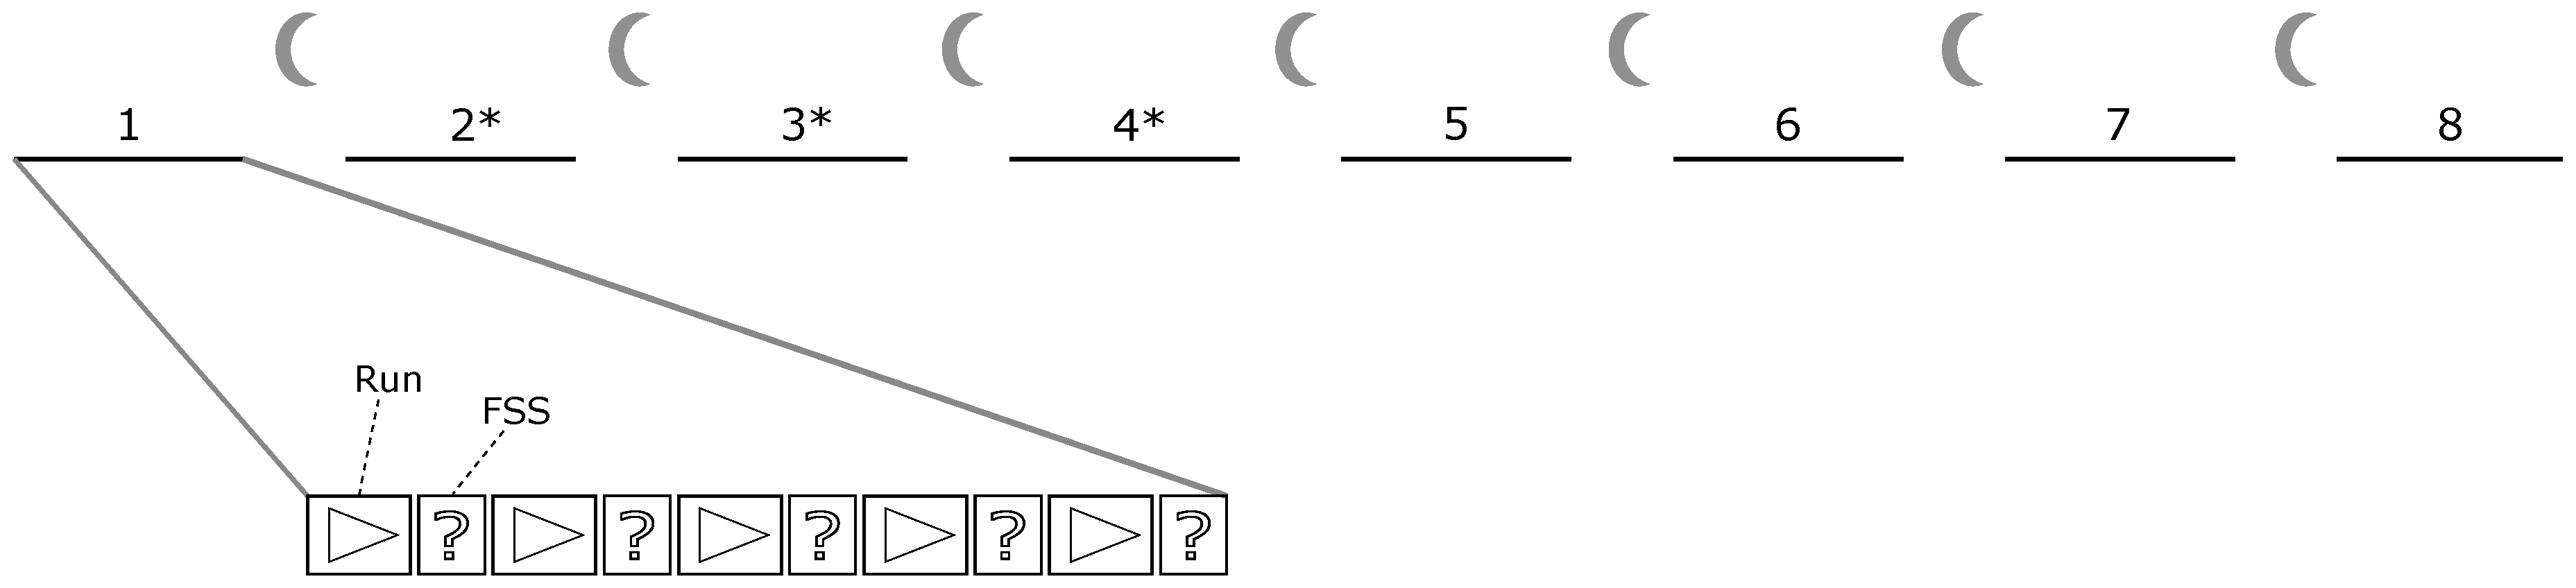
\includegraphics[width=\nicewidth]{design1}
\caption{The game was played in eight sessions on eight different days. In sessions 1 and 5--8, physiological signals were recorded during task performance; in session 2-4(*) no physiology was recorded. Each session consisted of five runs (2 to 4 min) followed by a self-report questionnaire (FSS, Flow Short Scale) about the latest run.}
\label{fig:design}
\end{figure*}

\subsection*{Materials}
\paragraph{Game.} The experimental task was a custom-made high-speed steering game {\it CogCarSim} designed specifically (by OL and JV) for the study of Flow and coded in Python (by JV). The participant steered a cube `avatar' moving forward along a straight track bounded by edges that could not be crossed.

The cube's side length was 2 units, and the track was 25 units wide. Stationary obstacles (red cones, red or yellow spheres with a height/diameter of 2 units) on the track had to be avoided. For each run, a total of 2,000 obstacles were placed randomly on the track, with placement constrained to always allow a path through. Track length varied between 24196.4 and 24199.7 units (mean 24197.8, sd 0.8). The speed of the cube was initially set to 1.6 units per step (96 units per second); increased at a constant rate (0.0012 units/step at every step); and slowed down if obstacles were hit (0.102 units/step at each collision). When a collision caused a speed drop, the screen flashed to indicate a collision; there followed an immunity period of 100 steps during which additional collisions did not cause speed drops. Participants could only affect speed indirectly, by controlling collisions. The participant was instructed to avoid as many obstacles they could in order to complete the run as fast as possible. The horizontal field of view angle of the virtual camera was 60 degrees and vertical 32 degrees. The camera was positioned behind the cube at 4 units height, pointing forward along the track.
% Speed was not direcly controlled by the participant, but instead increased linearly - starting each run from a predefined velocity of 1.6 units per step. Colliding with obstacles slowed the speed down by a constant increment (0.102 units), and the screen flashed indicating a collision.

The game had maximally simple one degree-of-freedom linear and holonomic dynamics: the horizontal position of the cube was directly proportional to steering wheel angle. Extensive self-piloting was done to adjust the graphics, e.g. virtual eye height; plus starting and increment speeds, rate of change of speed during collisions, and steering wheel sensitivity (steering ratio and damping).
% The steering had a very simple holonomic linear response dynamics (the lateral position of a cube `avatar' was directly proportional to steering wheel angle).

The participants started each run by pressing a button on the steering wheel when they felt ready. At the end of each run, the elapsed time and number of collisions were displayed, along with these statistics for the participant's ten best runs so far.

Data collected by CogCarSim included the positions, shape, and colour of obstacles on the track; run-level aggregated performance data (run duration, number of collisions, average velocity); and within-run time series data (steering wheel and cube position, speed, registered collisions).

\paragraph{Equipment.} The game was run on a Corsair Anne Bonny with Intel i7 7700k processor and an Nvidia GTX 1080 graphics card, running Windows 10. Eye-tracking and physiological signals were collected and stored on an Asus UX303L laptop with Debian GNU/Linux 9 OS.

The participant was seated in a Playseat Evolution Alcantara playseat (Playseats B.V., The Netherlands) aligned with the mid point of the 55" display screen (LG 55UF85). The screen resolution was 1920 x 1080 pixels, the frame rate was 60 and the refresh rate 60 Hz. The viewing distance was adjusted for each participant (so that they could place their hands on the steering wheel comfortably) and was approximately between 90 and 120 cm from the eye to the screen. The game was controlled wih a Logitech G920 Driving Force steering wheel (Logitech, Fremont, CA). Steering wheel settings in Logitech Gaming Software 8.96.88: sensitivity 100 percent, centering spring strength 4 percent, and wheel operating range 900 degrees.

Eye movements were measured using Pupil Labs Binocular 120 Hz eye tracker (Pupil Labs UG haftungsbeschränkt, Berlin, Germany), stabilised with a custom-built headband.
\todo[inline,author=BC]{MAYBEDO: Show Pupil, using picture by Mr. Rinkkala??}
Pupil Capture software was used to collect the data from the pupil hardware. Gaze direction was calibrated using ten markers on the display, a minimum of three times during the session. Additional calibrations were done if needed. Eye movement signal was recorded at 60 Hz.

For Electrodermal activity (EDA), Ag-AgCl electrodes with 0.5 saline paste were attached to the medial side of the left foot with adhesive skin tape and gauze. The plantar site was used instead of the palmar site to minimise artefacts resulting from the use of the steering wheel, as per guidelines by Boucsein (2012). Blood volume pulse (BVP) was measured using a pulse oximeter sensor attached to the left index toe of each participant. EDA and BVP were recorded at 128 Hz sampling rate using NeXus-10 (Mind Media B.V, Roermond-Herten, The Netherlands) connected to a laptop via bluetooth. The data was recorded using Trusas signal acquisition software, available open access at \url{https://github.com/jampekka/trusas-nexus}.


\paragraph{Flow Short Scale.} To measure self-reported Flow, participants were asked to fill in the Flow Short Scale (FSS) after each run \cite{Rheinberg2003,Engeser2008}. FSS has 10 core items which load the subfactors {\it fluency of performance} (6 items) and {\it absorption by activity} (4 items); plus 3 items for {\it perceived importance}. The response format of FSS is a 7-point Likert scale ranging from {\it Not at all} to {\it Very much}. Higher scores on the scales indicate higher experienced Flow and perceived importance. Example items include ``My thoughts/activities run fluidly and smoothly'' ({\it fluency of performance}), ``I do not notice time passing'' ({\it absorption by activity}), and ``I must not make any mistakes here'' ({\it perceived importance}). See Supplementary Information for full English text and Finnish translation.

Cronbach’s alpha for a 10-item scale including the {\it fluency of performance} and {\it absorption by activity} items was .92; Cronbach’s alpha was .87 for the 13-item FSS scale including {\it perceived importance} \cite{Rheinberg2003}. For our data also, Cronbach's alpha was higher for the core 10- than for 13-item scale. And FSS authors \cite{Rheinberg2003} suggest using the 10-item scale (excluding {\it perceived importance} subfactor) as a measure of experienced Flow. Thus, the Flow scale used in our analyses was formed by averaging the items in the {\it fluency of performance} and {\it absorption by activity} subfactors. The {\it perceived importance} subfactor was used separately in some analyses (see Results).

% (+3 additional items)
In addition to the 13 main items asked after every run, participants were asked at the end of every session to report 3 more items measuring the fit of skills and demands of the task (from  \cite{Rheinberg2003}. These items also had 7-point scales, e.g.: ``For me personally, the current demands are... (too low -- -- just right -- -- too high)''.

There was no Finnish translation of the scale available, so it was translated into Finnish by the authors. Two of the authors (native speakers of Finnish, no formal qualifications for English-Finnish translation) first made translations independently; these translations were compared and revised, then reviewed by other Finnish-native authors, and revised.

\subsection*{Procedure}
After recruiting, participants selected eight suitable dates within a three-week period. All sessions took place between 8 a.m. and 7 p.m. at Traffic Research Unit, Department of Digital Humanities, University of Helsinki. In the first session, participants were informed about the procedure of the study and asked to fill in a background information questionnaire, including information on health, driving experience and gaming experience, and an informed consent form.

The sessions were run by two research assistants at a time, who observed the measurement hidden out of participants' line of sight behind a partition wall, and took notes about possible confounding factors and problems within the session. In the beginning of each session participants filled in a session-wise questionnaire on the use of contact lenses, restedness, and medication, caffeine, and nicotine intake.

In  sessions 2 to 4 participants started played five runs straight after filling in the session-wise questionnaire. The FSS was filled after each run. In sessions with physiological measurements (1 and 5 to 8), participants were dressed in physiological sensors and an eye-tracking headset, seated in the driving seat in quiet, low-light conditions for baseline measurement. They were asked to sit still for five minutes, looking at a dark blue screen, while baseline was recorded. After baseline recording, participants played five game runs, filling FSS after each run. At the end of Session 8, the participants were debriefed and given the reward of culture vouchers.

\subsection*{Signal preprocessing and analysis}
Eye blinks were counted manually from the eye tracking videos recorded during baseline period of sessions 1 and 5--8. Three-minute periods were considered sufficient for this purpose, thus the first and last minute from each five-minute recording were omitted to obtain the most stable period of baseline. Four measurements (out of 40) were excluded, due to measurement problems.

All fast and simultaneous movements of both eyelids were counted as blinks (even if the eyelid did not fully close). To ensure reliable blink identification, two of the authors independently counted the number of blinks in sessions 1, 6 and 8, and inter-rater reliability of the counts was calculated as 98,7\% (see below). We considered this high enough to have blinks in remaining sessions 5 and 7 counted by only one experimenter.

We calculated the level of consensus between the two raters as follows. Separately for each participant and session, we divide the difference of two raters' blink counts by the mean of those counts, and then subtract the quotient from 1 to obtain a percentage. All percentages are then averaged to give the overall measure of inter-rater reliability. The session-wise reliability scores also had low variability (mean of standard deviations = 0.01).

The final spontaneous eye blink rate was calculated as median blinks per minute over baseline measurement sessions.


\subsection*{Statistical methods}
\textit{Describe any suitably concise and relevant stat methods here}

\todo[author=BC,inline]{JUSSI: Stats calculated for RQ2 were corrected for non-iid, by LMM models, explain}

\todo[author=OL,inline]{deviation scores are the residuals of the linear model in the log transformed coords, i.e. differences of logs in log(s)? units should be stated explicitly. also, difference of logs is ratio of performance (in seconds), so the same deviation in seconds has a bigger effect in the later runs, right? this is maybe sensible.}


%%%%%%%%%%%%%%%%%%%%%%%%%%%%%%%%%%%%%%%%%%%%%%%%%%%%%%%%%%%%%%%%%%%%%%%%%%%%%%%%
%%%%%%%%%%%%%%%%%%%%%%%%%%%%%%%%%%%%%%%%%%%%%%%%%%%%%%%%%%%%%%%%%%%%%%%%%%%%%%%%
%%%%%%%%%%%%%%%%%%%%% POST-HOC MATERIAL OF VITAL IMPORTANCE %%%%%%%%%%%%%%%%%%%%
\bibliography{cleanbib/CogCarFlow_bib}


\section*{Acknowledgements (not compulsory)}
Authors wish to thank Kalle Toikka for conceptual contributions, data gathering, and team-work.


\section*{Author contributions statement}
% please edit as appropriate
OL JP and BUC conceived the study.
OL and JV designed the gameplay.
JV implemented the game.
BUC and TT designed and implemented the data collection.
NL TT PP RF VPI and JP translated the FSS.
All authors participated in decisions on the experiment specifications.
RF VPI NL PP and TT conducted the experiment.
BUC VPI TT RF PP NL JP and OL analysed and interpreted the results.
BUC, JP and OL drafted the paper.
All authors participated in writing and reviewing, and approved the manuscript.


\section*{Additional information}
\wineAm{0.5}{1.0}{270}{10cm}{7cm}

The corresponding author is responsible for submitting a \href{http://www.nature.com/srep/policies/index.html#competing}{competing financial interests statement} on behalf of all authors of the paper. This statement must be included in the submitted article file.

\section*{Supplementary Information}

\subsection*{Flow Short Scale, in English with Finnish Translation}


\begin{table}[h]
\begin{tabular}{l p{0.4\textwidth} p{0.4\textwidth}}
\multicolumn{3}{l}{Core items of Flow: {\it fluency of performance} (2, 4, 5, 7, 8, 9) and {\it absorption by activity} (1, 3, 6, 10):} \\
\\
1. & I feel just the right amount of challenge    &    Peli tuntui juuri sopivan haastavalta  \\
2. & My thoughts/activities run fluidly and smoothly   & Pelasin sujuvasti \\
3. & I do not notice time passing  & En huomannut ajankulkua \\
4. & I have no difficulty concentrating & Pystyin hyvin keskittym\"{a}\"{a}n \\
5. & My mind is completely clear & Mieleni oli selke\"{a} \\
6. & I am totally absorbed in what I am doing & Uppouduin t\"{a}ysin pelaamiseen \\
7. & The right thoughts/movements occur of their own accord & L\"{o}ysin oikeat liikkeet kuin itsest\"{a}\"{a}n \\
8. & I know what I have to do each step of the way & Olin koko ajan tilanteen tasalla \\
9. & I feel that I have everything under control & Tunsin hallitsevani tilannetta \\
10. & I am completely lost in thought & Syvennyin peliin t\"{a}ysin  \\
\\
\multicolumn{3}{l}{Extra items for {\it perceived importance}:} \\
\\
11. & Something important to me is at stake here & Koin peliss\"{a} onnistumisen t\"{a}rke\"{a}ksi \\
12. & I must not make any mistakes here & Minusta tuntui silt\"{a}, etten saisi tehd\"{a} yht\"{a}k\"{a}\"{a}n virhett\"{a}\\
13. & I am worried about failing & Pelk\"{a}sin ep\"{a}onnistuvani\\
\\
\multicolumn{3}{l}{Extra items for the fit of skills and demands:} \\
\\
14. & Compared to all other activities which I partake in,this one is... (easy/difficult) & Verrattuna muihin tekemiini asioihin, t\"{a}m\"{a} on... (helppoa/vaikeaa) \\
15. & I think that my competence in this area is... (low/high)  & Osaamiseni taso on... (matala/korkea)\\
16. & For me personally, the current demands are... (too low/just right/too high) & Pelin vaativuus on t\"{a}ll\"{a} hetkell\"{a} minulle... (liian matala/sopiva/liian korkea)\\
\end{tabular}
\end{table}


\subsection*{Descriptive Statistics and Visuals}

\begin{minipage}{\textwidth}
\centering
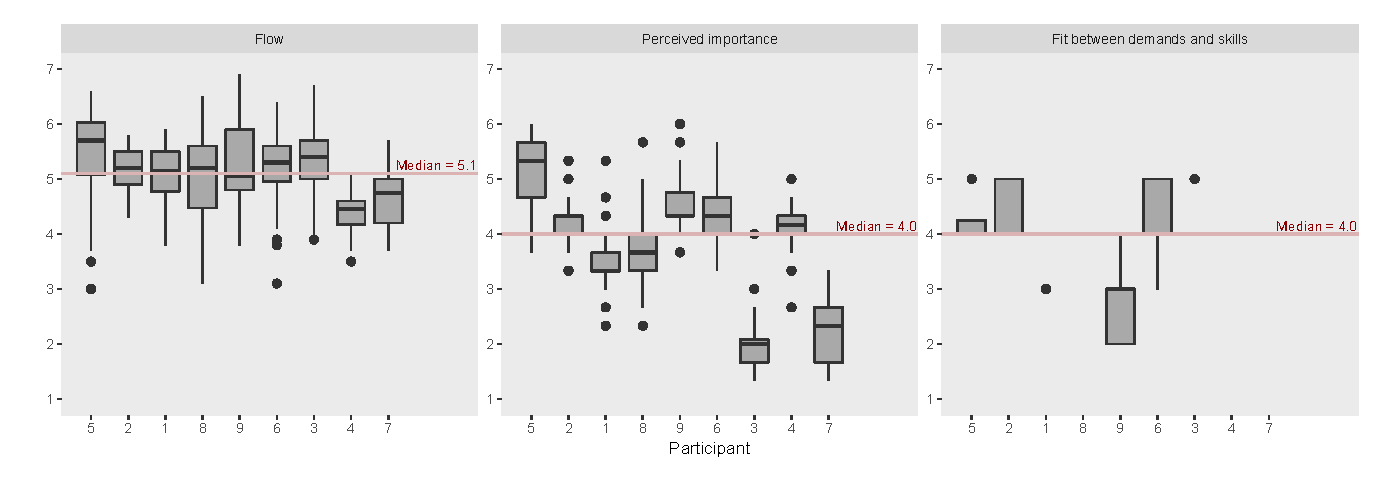
\includegraphics[width=\linewidth]{suppl_fss_boxplots}
\captionof{figure}{Boxplots for Flow Short Scale measures by participant in order of game performance (mean run duration).}
\label{fig:supp_boxes}
\end{minipage}%

\begin{minipage}{\textwidth}
\centering
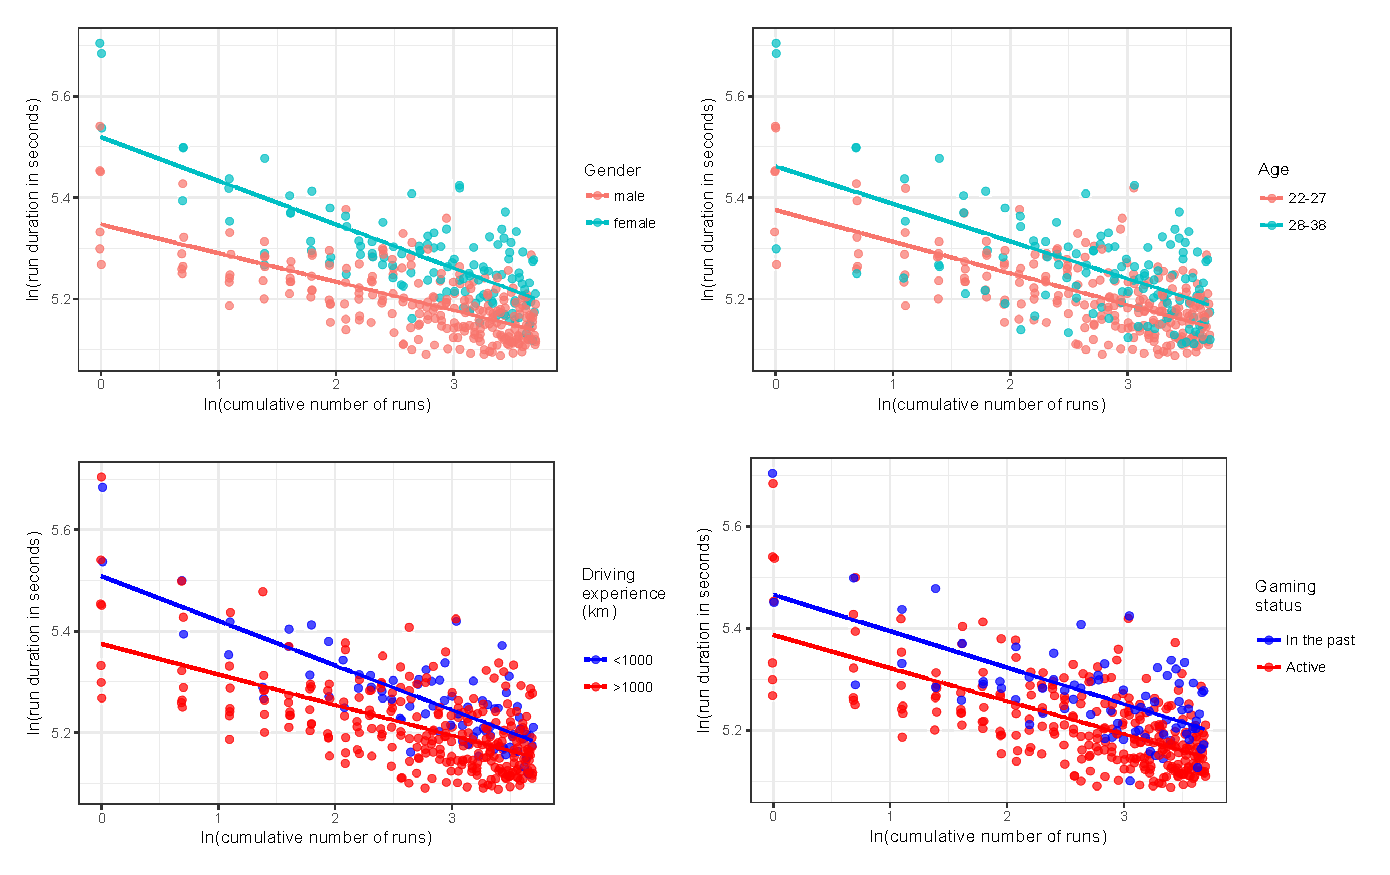
\includegraphics[width=\linewidth]{suppl_learningcurve_groups}
\captionof{figure}{Log-log graphs for cumulative runs and run duration with different grouping factors (gender, age, driving experience, gaming experience.}
\label{fig:supp_LC_groups}
\end{minipage}%

\noindent
\begin{minipage}{\textwidth}
\begin{minipage}{.6\textwidth}
\centering
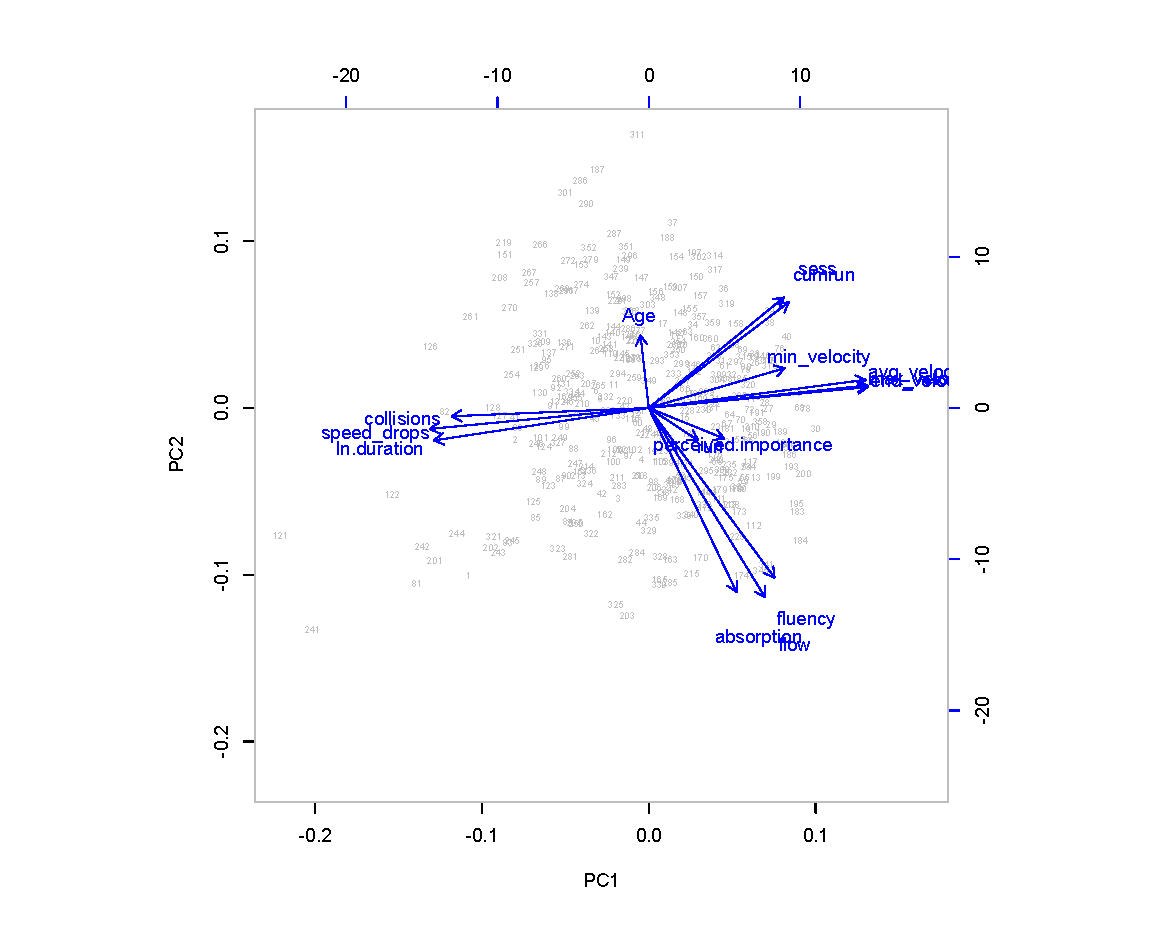
\includegraphics[width=\linewidth]{suppl_pca}
\label{fig:supp_boxes}
\end{minipage}% This must go next to `\end{minipage}`
\begin{minipage}{.4\textwidth}
\begin{tabular}{lll}
{\bf Variable}   &{\bf PC1}&{\bf PC2}\\
\hline
run              & 0.801  & -0.088 \\
min\_velocity    & 0.221  & 0.109  \\
max\_velocity    & 0.356  & 0.062  \\
end\_velocity    & 0.356  & 0.057  \\
avg\_velocity    & 0.353  & 0.076  \\
collisions       & -0.321 & -0.023 \\
speed\_drops     & -0.356 & -0.057 \\
cumrun           & 0.228  & 0.289  \\
age              & -0.134 & 0.198  \\
fss\_fluency     & 0.204  & -0.464 \\
fss\_absorption  & 0.143  & -0.502 \\
perc. importance & 0.122  & -0.083 \\
Flow             & 0.189  & -0.517 \\
session          & 0.219  & 0.302  \\
ln.duration      & -0.349 & -0.089
\end{tabular}
\end{minipage}
\captionof{figure}{Summary of principal component analysis results: {\it Left panel} Biplot of principal components (PCs) 1 and 2; {\it Right panel} Component loadings for PC1 and PC2.}
\end{minipage}


\begin{table}[!h]
\centering
\caption{\label{tab:FluencyAbsorption}Descriptive statistics for fluency of performance and absorption by activity for each participant.}
\begin{tabular}{lllllll}
\hline
           & Participant & Mean & Median & SD   & Min  & Max  \\
\hline
Fluency    &             &      &        &      &      &      \\
           & 1           & 4.93 & 5.00   & .62  & 3.17 & 6.00 \\
           & 2           & 4.90 & 4.83   & .47  & 3.83 & 5.67 \\
           & 3           & 4.90 & 5.00   & .84  & 3.00 & 6.67 \\
           & 4           & 4.10 & 4.00   & .56  & 3.00 & 5.33 \\
           & 5           & 5.15 & 5.50   & 1.01 & 2.67 & 6.50 \\
           & 6           & 5.11 & 5.25   & .92  & 2.83 & 6.50 \\
           & 7           & 4.35 & 4.33   & .58  & 3.17 & 5.50 \\
           & 8           & 4.74 & 5.00   & .92  & 2.50 & 6.33 \\
           & 9           & 5.24 & 5.00   & .86  & 3.33 & 7.00 \\
\hline
Absorption &             &      &        &      &      &      \\
           & 1           & 5.37 & 5.50   & .45  & 4.25 & 6.25 \\
           & 2           & 5.60 & 5.75   & .37  & 5.00 & 6.00 \\
           & 3           & 6.04 & 6.00   & .43  & 5.25 & 6.75 \\
           & 4           & 4.85 & 4.88   & .39  & 4.00 & 5.75 \\
           & 5           & 5.89 & 6.0    & .80  & 3.50 & 7.00 \\
           & 6           & 5.37 & 5.50   & .74  & 3.50 & 6.75 \\
           & 7           & 5.19 & 5.25   & .54  & 4.25 & 6.25 \\
           & 8           & 5.24 & 5.50   & .95  & 3.00 & 6.75 \\
           & 9           & 5.27 & 5.13   & .72  & 4.00 & 6.75 \\
\hline
\end{tabular}
\end{table}


\begin{table}[!h]
\centering
\caption{\label{tab:GameVariables}Descriptive statistics of the game performance measures.}
\begin{tabular}{lllllll}
\hline
Variable & Description & Mean & Median & SD & Min & Max \\
\hline
min\_velocity & Minimum velocity of a run & 1.58 & 1.6 & 0.06 & 1.06 & 1.6 \\
max\_velocity & Maximum velocity of a run & 2.82 & 2.81 & 0.36 & 1.62 & 3.6 \\
end\_velocity & End velocity of a run & 2.72 & 2.78 & 0.4 & 1.14 & 3.59 \\
avg\_velocity & Mean velocity of a run & 2.23 & 2.26 & 0.19 & 1.37 & 2.54 \\
Collisions & Number of collisions in a run & 17.81 & 17 & 6.59 & 5 & 40 \\
speed\_drops & Number of speed drops in a run & 12.57 & 12 & 3.96 & 4 & 28 \\
duration & Duration of a run (s) & 186.07 & 181.99 & 18.24 & 162.15 & 300.1 \\
\hline
\end{tabular}
\end{table}


\todo[author=BC,inline]{Hi-res version needed!}
\begin{minipage}{\textwidth}
\centering
\includegraphics[width=\nicewidth]{variableMatrix}
\captionof{figure}{A scatterplot matrix of game performance measures. The diagonal of the matrix displays distributions (histograms) of each measure. The lower off-diagonal cells contain scatterplots, with loess-smoothed fit, of two measures from the corresponding row and column on the diagonal (panel above on the x-axis; panel to right on y-axis). The upper off-diagonal cells display corresponding Pearson correlation coefficients.}
\label{fig:scatter_matrix}
\end{minipage}

\subsection*{Additional Statistical Analyses}

\todo[author=BC,inline]{JUSSI: The permutation method...}

\todo[author=BC,inline]{MAYBEDO: Add Ville's whole model-fitting section of the report???}

\end{document}
